Em sistemas de geração fotovoltaica, a energia solar captada pelos painéis é convertida em energia elétrica em corrente contínua.
Como a maioria desses sistemas não possui meios de armazenamento, e como energia se conserva, toda a energia gerada
pelos painéis deve ser imediatamente injetada na rede elétrica.

Para escoar essa produção, os inversores devem não apenas executar a conversão CC--CA, mas fazê--la de forma
a controlar a injeção de potência na rede, garantindo o equilíbrio energético e consequentemente a estabilidade do
barramento CC.

Para isso, a tensão imposta pelo inversor deve estar em sincronismo com a da rede.
O controle da potência ativa depende diretamente da defasagem entre a tensão da rede e a tensão imposta pelo inversor.
Além disso, como a rede elétrica opera com frequência variável em torno dos 60 Hz, o inversor deve estimar
continuamente a fase da tensão da rede a fim de realizar os ajustes necessários para manter o sincronismo e o
ângulo de carga desejado.

Essa estimação não é trivial já que, além das variações da tensão e frequência em regime permanente, a rede ainda
apresenta efeitos transitórios impulsivos e oscilatórios, distorções harmônicas, flutuações, ruídos, afundamentos, etc.
Isso é ainda mais desafiador em sistemas monofásicos, onde amplitude, frequência e fase devem ser obtidas a partir de
medições de um único sinal de tensão, sujeito aos fenômenos já citados.

Na prática, existem algumas estratégias para se obter uma estimativa instantânea e precisa da fase da tensão da rede,
sendo que a maioria delas é baseada na estrutura SOGI--PLL, cujo diagrama de blocos básico é apresentado na \figr{fig:ex01}.
\begin{figure}[htbp]
    \centering
    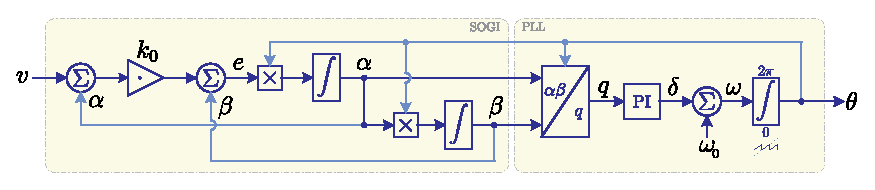
\includegraphics{figs/pll.eps}
    \caption{SOGI--PLL.}
    \label{fig:ex01}
\end{figure}



O estimador da \figr{fig:ex01} pode ser discretizado e reescrito na forma de equações a diferenças, apresentadas nas equações
(\ref{eq:0}--\ref{eq:6}), possibilitando sua implementação em controladores digitais embarcados.

O algoritmo discretizado recebe um sinal amostrado da tensão de entrada --- tipicamente com frequência de amostragem
na ordem de algumas dezenas de kHz, dependendo da frequência de comutação utilizada no inversor.

Com base nessas amostras, estima-se a fase da tensão quase instantânea (com atraso de uma amostra).
O sinal de fase estimado é utilizado nas malhas de controle das correntes e potências ativa e reativa injetadas na rede
(não abordados nessa questão).
\begin{equation}\label{eq:0}
        e\0 = k_{_0\!} \left( v\0 - \alpha\1 \right)  - \beta\1
\end{equation}
\begin{equation}\label{eq:1}
    \alpha\0 = w\1  \, k_{_1}  \left( e\0 + e\1 \right)  + \alpha\1
\end{equation}
\begin{equation}\label{eq:2}
    \beta\0 = w\1  \, k_{_1}  \left( \alpha\0 + \alpha\1 \right)  + \beta\1
\end{equation}
\begin{equation}\label{eq:3a}
    d{_{_{ n\!}}} =  \alpha\0 \sin(\theta\1) - \beta\0  \cos(\theta\1)
\end{equation}
\begin{equation}\label{eq:3b}
    q{_{_{ n\!}}} =  \alpha\0 \cos(\theta\1) + \beta\0  \sin(\theta\1)
\end{equation}
\begin{equation}\label{eq:4}
    \delta\0 = k_{_2} q{_{_{ n\!}}} + k_{_3} q{_{_{ n\text{-}\!\>\!1\!}}} + \delta\1
\end{equation}
\begin{equation}\label{eq:5}
    \omega\0  = \omega_{_0} + \delta\0
\end{equation}
\begin{equation}\label{eq:6}
    \theta\0 = k_{_1}  \left( \omega\0 + \omega\1 \right)  + \theta\1    \ \ \  (\text{mod}~2\pi)
\end{equation}

A estimativa de fase da rede ($theta$) obtida ainda deve ser validada.
O \inlcode{pll} pode demorar alguns ciclos para se sincronizar com a rede (ou atracar).


\section*{Tarefa 1}
Em \colorurl{https://github.com/j-Lago/pythonTutorial/blob/master/data/grid_voltage.csv} você encontrará um
arquivo \colorurl{grid_voltage.csv} com a
tensão (\textbf{coluna 2}) amostrada de alguns ciclos da rede elétrica e um registro temporal (\textbf{coluna 1}) de cada amostra.

Escreva um script que importe esse sinal para um \inlcode{array}, e para cada amostra (cada elemento do \inlcode{array})
execute os cálculos (\ref{eq:0}--\ref{eq:6}).
Guarde os resultados de cada amostra de $v$ (tensão de entrada), $\alpha$ (tensão filtrada), $d$ (componente de eixo
direto da tensão em base síncrona), $q$ (componente em quadratura) e $\theta$ (fase estimada pelo PLL).

Assuma ainda, de forma simplificada, que o sincronismo foi obtido no instante do primeiro cruzamento por zero do sinal
$\theta$ (saída do PLL) em que $\arctan(q/d) < 0.02$~rad ($\approx 2^\circ)$ e $d > 250$~V. Identifique esse instante
bem como os demais cruzamentos por zero subsequentes.

Utilize as seguintes constantes para a implementação do controlador e das integrações:
\begin{equation}\label{eq:cont}
    \begin{aligned}
        k_{_0} &= 0.7 \\
        k_{_1} &= 2.84\cdot 10^{-6} \\
        k_{_2} &= 0.385715277950311 \\
        k_{_3} &= -0.385713293478261 \\
        \omega_{_0} &= 376.9911184307752
    \end{aligned}
\end{equation}

Gere e exporte uma figura apresentado a evolução temporal de cada uma desses sinais, bem como alguma indicação do
instante que o PLL conseguiu se sincronizar (atracar) com a rede elétrica.
A \figr{fig:plot} mostra um exemplo de como os resultados do script podem ser
apresentados.
\begin{figure}[htbp]
    \centering
    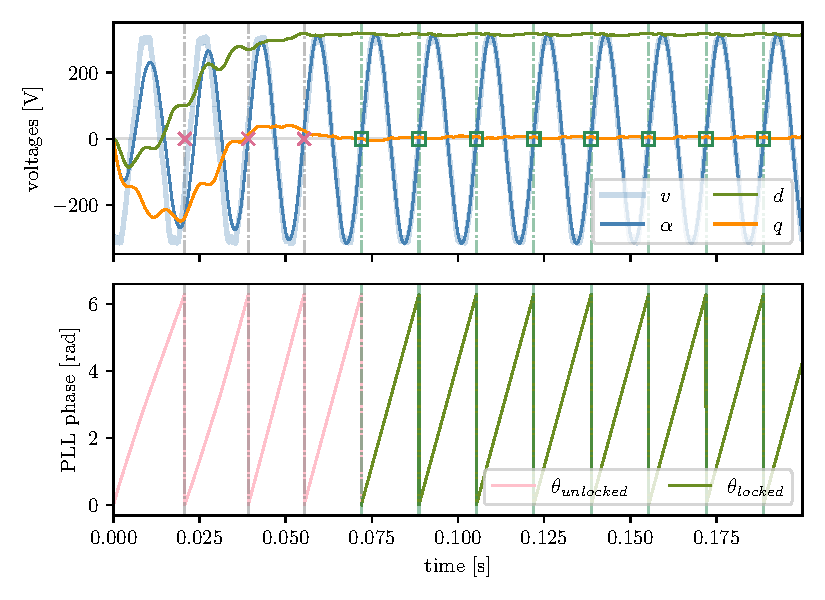
\includegraphics[scale=1.0]{figs/plot_pll}
    \caption{Resultado esperado do script.}
    \label{fig:plot}
\end{figure}




\section*{Tarefa 2}
Exporte para um arquivo \inlcode{.csv} a porção do sinal de tensão de entrada compreendida entre a detecção
inicial da sincronização até a amostra que antecede o último cruzamento por zero do ângulo $\theta$, ou seja, o período
que compreende todos os ciclos inteiros em que o PLL estava sincronizado.
Exporte além da tensão, o período correspondente do vetor de tempo e do ângulo de saída do PLL.
%\begin{table}[]
%    \centering
%    \small
%    \texttt{
%        \begin{tabular}{%{lll}
%                >{\columncolor{lightgray}}l
%                >{\columncolor{lightgray}}l
%                >{\columncolor{lightgray}}l }
%            time,  & phase,  & voltage              \\
%            0.12562,  & 0.001584790,  & 4.3073               \\
%            0.12562,  & 0.003702030,  & 14.323               \\
%            0.12563,  & 0.005819309,  & -0.32799             \\
%            0.12564,  & 0.007936621,  & 14.62                \\
%            0.12564,  & 0.010053976,  & 14.767								\\
%            $\ \ \ \ \vdots$     & \ \ \ \ \ \ $\vdots$            & \ \ \  $\vdots$\\
%            0.19247,  & 6.280264753,  & 10.071
%        \end{tabular}
%    }
%    \caption{Exemplo da tabela a ser exportada em formato \texttt{.csv}.}
%    \label{tab:csv}
%\end{table}


\pagebreak

\begin{minted}[escapeinside=??, frame=single, rulecolor=brown, bgcolor=bgcsv]{output}
?\textcolor{brown}{\faIcon{file} amostras\_sincronizadas.csv}?
\end{minted}
\vspace{-0.8em}
\begin{minted}[escapeinside=??, bgcolor=bgcsv]{output}
time,    phase,       voltage
0.12562, 0.001584790, 4.3073
0.12562, 0.003702030, 14.323
0.12563, 0.005819309, -0.32799
0.12564, 0.007936621, 14.62
0.12564, 0.010053976, 14.767
    :         :          :
0.19247, 6.280264753, 10.071
\end{minted}


\section*{Tarefa 3}
Os dados exportados na tarefa anterior consistem num intervalo da tensão da rede com ciclos inteiros.
Isso nos permite calcular o valor rms da tensão amostrada da rede através de \eqr{eq:rms}:
\begin{equation}\label{eq:rms}
V_{\text{rms}} = \sqrt{\dfrac{1}{N} \sum_ {n=0} ^{N-1} v\0 ^2}
\end{equation}

Escreva uma função  \inlcode{rms(path: str) -> tuple[float, float]} que recebe como argumento um texto indicando o caminho
do arquivo exportado na questão anterior e que calcule e retorne o valor rms da tensão e sua frequência fundamental média.
\begin{minted}{custompython}
def rms(path: str) -> tuple[float, float]:
    # seu código aqui

vrms, f1 = rms('amostras_sincronizadas.csv')
print(f"A amostra de tensão possui valor rms de {vrms:.2f} V e frequência {f1:.2f} Hz")
\end{minted}

Saída esperada:
\begin{minted}{text}
A amostra de tensão possui valor rms de 220.93 V e frequência 59.84 Hz
\end{minted}

$^\dagger$\emph{Note que \eqr{eq:rms} só é válida para um vetor $\mathbf{x}$ contendo ciclos inteiros da componente fundamental.
Ainda, para melhorar a precisão do método, recomenda-se realizar o cálculo considerando ao menos dez ciclos completos da fundamental.
    (o que não é possível nesse exemplo pelo tamanho da amostra inicial)}


